\documentclass[11pt,a4paper]{article}
\usepackage[margin=24mm,top=23mm,bottom=24mm]{geometry}
\usepackage[T1]{fontenc}
\usepackage[utf8]{inputenc}
\usepackage{lmodern,microtype}
\usepackage{amsmath,amssymb,mathtools}
\usepackage{graphicx,booktabs,tabularx,array,longtable,multirow}
\usepackage[table]{xcolor}
\usepackage{caption,float}
\usepackage{enumitem}
\usepackage{fancyhdr,lastpage}
\usepackage{hyperref}
\hypersetup{colorlinks=true,linkcolor=blue!55!black,urlcolor=blue!50!black,citecolor=blue!50!black,pdftitle={Reliable Estimation of Missed Harmful Responses: Human-Label Uncertainty and Review Costs},pdfauthor={Tivdzua Lubem Noah}}
\definecolor{navy}{HTML}{17354E}
\definecolor{teal}{HTML}{317D8B}
\definecolor{pale}{HTML}{EAF0F3}
\definecolor{graytext}{HTML}{4A5560}
\renewcommand{\arraystretch}{1.13}
\setlength{\parskip}{2.3pt}
\setlength{\parindent}{0pt}
\setlist[itemize]{topsep=4pt,itemsep=2pt,parsep=0pt,leftmargin=18pt}
\setlist[enumerate]{topsep=4pt,itemsep=2pt,parsep=0pt,leftmargin=18pt}
\captionsetup{font=small,labelfont=bf,justification=raggedright,singlelinecheck=false}
\pagestyle{fancy}
\fancyhf{}
\fancyhead[L]{\footnotesize\textcolor{navy}{TRUSTWORTHY AI \;|\; TECHNICAL REPORT}}
\fancyhead[R]{\footnotesize\textcolor{graytext}{13 NOVEMBER 2026}}
\fancyfoot[L]{\footnotesize\textcolor{graytext}{Missed-harm estimation \;|\; empirical analysis}}
\fancyfoot[R]{\footnotesize\textcolor{graytext}{\thepage/\pageref{LastPage}}}
\renewcommand{\headrulewidth}{0.4pt}
\newcommand{\Y}{\ensuremath{Y}}
\newcommand{\D}{\ensuremath{D}}
\newcommand{\A}{\ensuremath{A}}
\newcommand{\Z}{\ensuremath{Z}}
\newcommand{\source}[1]{\textcolor{graytext}{\footnotesize\textit{Source: #1.}}}
\begin{document}
\begin{center}
{\small\scshape INNOPOLIS UNIVERSITY \;\textbar\; TRUSTWORTHY AI RESEARCH}\\[9mm]
{\Huge\bfseries\color{navy} Reliable Estimation of\\[1mm] Missed Harmful Responses}\\[4mm]
{\Large\color{graytext} Human-label uncertainty and cost-aware statistical estimation}\\[8mm]
{\large\bfseries Research results and statistical analysis}\\[3mm]
{\normalsize Lubem Noah Tivdzua}\\[2mm]
{\small 13 November 2026}
\end{center}
\vspace{6mm}
\begin{abstract}
We study the prevalence of harmful assistant responses that pass a runtime safety monitor, $A=P(Y=1,D=0)$, where $Y$ denotes response-level policy harm and $D=0$ denotes an allowed response. The analysis combines historical monitor decisions, a blinded human-review study of 96 cases and 336 assessments, and cost-matched comparisons of sampling and prediction-powered estimators. In a 1,687-response development comparison, selective Qwen acquisition reduced the number of historically labeled harmful allowed responses from 229 to 228. At a budget of 160 historical-label evaluations, allowed-only simple random sampling achieved RMSE 0.02369, compared with 0.02542--0.03552 for the tested StratPPI mean designs. Simulations using empirical review durations show that gains under error-free labeling can disappear when reviewers make independent or correlated errors. The human study also found substantial disagreement (Fleiss' $\kappa=0.3082$), limiting the interpretation of any single set of ratings as reference truth. We examine interval coverage, allocation optimization and recorded inference costs, and outline a small prospective validation study. The present results support further investigation of reference-label reliability and review efficiency; they do not establish the prevalence of latent harm in a fresh deployment population.
\end{abstract}
\vspace{3mm}

\section{Study scope and evaluation design}
The analysis concerns harmful responses that were allowed by a fixed runtime monitor. We first examine the historical effect of selective stronger-monitor acquisition, then evaluate agreement among independent human reviewers and the time required for those assessments. We compare simple random sampling with prediction-powered estimation methods under stated label and proxy-acquisition budgets. Finally, we examine how reviewer errors affect estimation and confidence intervals. All experiments use historical development data or simulated outcomes; no prospective reference-labeled deployment sample is included.

\begin{table}[H]\centering\small
\caption{Data and analyses used in this report.}
\begin{tabularx}{\textwidth}{@{}p{0.35\textwidth}p{0.26\textwidth}X@{}}\toprule
Component & Available evidence & Limitation\\\midrule
Historical monitor decisions & 1,687 response records & Historical, unverified harm labels\\
Independent human review & 96 cases; 336 assessments & No external reference standard\\
Sampling and PPI comparisons & Historical benchmarks and simulated populations & Some published methods implemented as restricted variants\\
Resource measurement & Human active times and recorded model latency & Economic conversion assumed\\
Interval and allocation checks & Simulation coverage and optimizer certificates & Does not validate latent-harm coverage\\
Prospective validation design & Sampling and adjudication protocol & Data collection has not begun\\\bottomrule
\end{tabularx}
\end{table}

\section{Target estimand and study population}
Let $(X,R)$ denote the prompt and the generated assistant response, respectively; $Y=1$ if the \emph{response} materially violates at least one category of the fixed C1--C8 response-level policy in context. A safe refusal to an unsafe prompt is $Y=0$. The frozen runtime monitor emits $D\in\{0,1\}$, where $D=0$ means ``allow'' and $D=1$ means ``block''; the monitor acts \emph{after} the response is generated and \emph{before} it is shown to the user. Our primary parameter is
\begin{equation}\label{eq:estimand}
 A=P(Y=1,D=0)=q\,p,\qquad q=P(D=0),\quad p=P(Y=1\mid D=0).
\end{equation}
The false-negative rate is different: $\mathrm{FNR}=A/P(Y=1)$ whenever $P(Y=1)>0$. The blocked-harm count contributes to the FNR denominator but not the primary missed-harm numerator. This distinction explains why a change in blocked cases can make FNR appear different without delivering a comparable reduction in $A$.

\textbf{Population scope.} The permitted historical development view comprises $N=1{,}687$ prompt--response cases: $N_0=1{,}557$ allowed ($q=0.92294$) and $N_1=130$ blocked. The sources are WildGuardTest, JailbreakBench judge-comparison and XSTest-safe. These are retrospectively assembled, not fresh native-monitor deployment examples. Source/family dependence and previously used test sets prevent confirmatory transport claims [D1].

\section{Historical effect of selective Qwen acquisition}
We separated allowed and blocked harmful responses to examine the historical effect of adding Qwen to the rule-plus-compact monitor. The archival label counts are summarized in Table~\ref{tab:qwen} [A1]:
\begin{table}[H]\centering
\caption{Harm-labeled responses by monitor decision in the historical development comparison.}\label{tab:qwen}
\begin{tabular}{@{}lrrr@{}}\toprule
Historical labeled class & Before Qwen & After Qwen & Change\\\midrule
Harmful and allowed & 229 & 228 & $-1$\\
Harmful and blocked & 62 & 63 & $+1$\\
Total labeled harmful & 291 & 291 & $0$\\\midrule
Apparent $A$ on $N=1{,}687$ & 0.13574 & 0.13515 & $-0.000593$\\\bottomrule
\end{tabular}
\end{table}
Thus the historical apparent improvement in $A$ is \emph{one case per 1,687}, i.e. $0.0593$ percentage points. This decomposition must not be interpreted as proof of a statistically meaningful or prospectively robust native-guard benefit. The earlier v2 routing proposal also had no jointly feasible development operating point and remains a \textbf{no-go}; four-guard screening failures are retained as negative evidence [D1].

\section{Human-review study}
\subsection{Design and descriptive results}
The subsequent historical study sampled 96 cases across source and archived monitor-decision strata. R1, R2 and R3 each judged all 96 cases independently; R4 evaluated 48 selected cases (39 disagreements/uncertainties plus 9 audited unanimous cases), for $288+48=336$ total judgments. The label set included \texttt{safe}, \texttt{harmful} and \texttt{uncertain}; prompt harmfulness did not define response harmfulness. The fourth-rater sample was \emph{selected}, not a random 48-case reference standard [A2].
\begin{table}[H]\centering\small
\caption{Aggregate observations from the real historical reviewer study [A2].}
\begin{tabular}{@{}lrrrr@{}}\toprule
Measure & R1 & R2 & R3 & R4 (selected)\\\midrule
Cases reviewed & 96 & 96 & 96 & 48\\
Harmful votes & 10 & 38 & 15 & 14\\
Safe votes & 74 & 57 & 76 & 34\\
Uncertain votes & 12 & 1 & 5 & 0\\
Active seconds & 3,810.5 & 3,715.9 & 4,264.1 & 4,054.5\\
Mean active sec / vote & 39.69 & 38.71 & 44.42 & 84.47\\\bottomrule
\end{tabular}
\end{table}
Primary vote patterns: 57/96 binary-unanimous, 21/96 binary 2:1, and 18/96 containing at least one Uncertain vote. Fleiss' three-category $\kappa=0.3082$, with pairwise raw agreement $0.7014$; this describes \emph{agreement}, not correctness. The source/decision-weighted apparent missed-harm quantities among allowed cases, with uncertain labels excluded, were \textbf{R1 0.0554, R2 0.3116, R3 0.1222}. These are different reviewer-defined endpoints; none is a verified estimate of latent $A$.

\subsection{Review time}
Recorded browser-active time totaled \textbf{15,844.87 s} ($4.40$ h); wall time totaled \textbf{23,638.05 s} ($6.57$ h). R4 accounted for $4{,}054.46$ active seconds (25.59\% of total). Across all 336 actions, mean recorded active duration was $47.16$ s, with maximum recorded duration $206.50$ s [A2]. Browser-active time does not measure concentration perfectly; wall time includes interruptions. R4's higher time is confounded by the selected case difficulty and cannot be attributed causally to fourth-reviewer status. These measurements do not include recruitment, training or organizer time.

\section{Misclassification and identifiability}
Let $Z$ denote a binary \emph{reviewer-defined} response-harm verdict, with conditional sensitivity $s=P(Z=1\mid Y=1,D=0)$ and specificity $t=P(Z=0\mid Y=0,D=0)$. Under homogeneous misclassification for illustration,
\begin{align}
 A_Z&=P(Z=1,D=0)=q\bigl[sp+(1-t)(1-p)\bigr],\\
 A_Z-A&=q\bigl[(1-t)+(s+t-2)p\bigr].\label{eq:bias}
\end{align}
For example, with assumed $s=0.80$ and $t=0.96$, bias equals $q(0.04-0.24p)$, which does \emph{not} vanish with a larger review sample. If $s,t$ were known with $s+t>1$, one could algebraically invert to $p=(A_Z/q+t-1)/(s+t-1)$, subject to estimation error and calibration uncertainty. \emph{Those rates are not known from the current study.}

Nonidentification without assumptions is immediate: the same observed distribution of $Z$ is compatible with (a) $Y=Z$ and (b) a latent $Y$ independent of $Z$ at any prevalence $p$. Adding correlated or selectively sampled reviewers does not eliminate this ambiguity without identifying restrictions. The three-binary-rater conditionally independent two-class model is just identified (7 observed degrees of freedom, 7 latent parameters) and cannot be validated simply by a residual goodness-of-fit test; dropping \texttt{uncertain} changes the analyzed case population [A2]. The argument follows standard results on misclassification and latent-class identification.

\section{Sampling baselines and sensitivity to reviewer errors}
\subsection{Historical 160-label comparison}
The historical comparison evaluates agreement with historical \emph{unverified} labels at a fixed budget of 160 label evaluations. Pilot tuning judgments were charged within that budget [A1].
\begin{table}[H]\centering\small
\caption{Historical development comparison: RMSE against historical labels, not validated policy truth.}
\begin{tabular}{@{}lrr@{}}\toprule
Estimator & Calibration labels & RMSE\\\midrule
Allowed-only simple random sampling & 0 & \textbf{0.02369}\\
Proportional StratPPI mean, fixed $\lambda=1$ & 0 & 0.02542\\
Proportional StratPPI mean, pilot-tuned $\lambda$ & 32 & 0.02936\\
Allowed-heavy StratPPI mean, pilot-tuned $\lambda$ & 32 & 0.03552\\\bottomrule
\end{tabular}
\end{table}
A related restricted active-PPI study exceeded its \emph{realized} hypothetical time budget in 49\% of its runs and had no established improvement. A method that fails a realized cost gate cannot be characterized as a hard-budget winner. None of these restricted mean designs is a complete author-paper implementation.

\subsection{Repeated human reviews under simulated error}
Separate simulations generated \emph{16 independent latent populations per geometry}, with repeated measurement actions at a common $4{,}800$ active-second budget. The selected comparison below uses the single allowed-only reviewer, equal proxy-stratification, and three-vote majority. All values measure error against synthetic latent $Y$; majority votes are not factual gold labels in the actual study.
\begin{table}[H]\centering\scriptsize
\caption{Synthetic latent-$Y$ RMSE, 4,800 review-active-second budget (smaller is better).}
\begin{tabular}{@{}llrrr@{}}\toprule
Population geometry & Reviewer model & Allowed SRS & Proxy-stratified & Three-vote majority\\\midrule
1,687 & perfect binary & 0.0123 & 0.0068 & 0.0229 \\
1,687 & noisy independent & 0.0364 & 0.0368 & 0.0226 \\
1,687 & noisy correlated & 0.0709 & 0.0765 & 0.0507 \\
1,687 & correlated with abstention & 0.0937 & 0.0942 & 0.0600 \\
5,000 & perfect binary & 0.0115 & 0.0068 & 0.0197 \\
5,000 & noisy independent & 0.0306 & 0.0334 & 0.0214 \\
5,000 & noisy correlated & 0.0609 & 0.0634 & 0.0444 \\
5,000 & correlated with abstention & 0.0807 & 0.0810 & 0.0494 \\
\bottomrule\end{tabular}
\end{table}
With perfect synthetic labels, proxy stratification performs well; when simulated raters disagree, repeat judgments may lower error against simulated truth even though they reduce the number of distinct cases reviewed. The advantage is \emph{scenario-dependent}: it does not validate majority voting as a ground-truth method. Costs and reference correctness must be separated.

\section{Cost-matched comparison of estimators}
\subsection{Simulation design and methodology}
The cost-matched benchmark evaluates six algorithms: whole-population SRS, allowed-only SRS, pilot-tuned PPI++ mean specialization, StratPPI mean specialization, MultiPPI subset-GLS restricted adaptation, and a restricted active augmented inverse-propensity-weighted (AIPW) method [A3]. Each experiment uses one of two synthetic population geometries, $N=1{,}687$ ($N_0=1{,}557$) or $N=5{,}000$ ($N_0=4{,}000$); eight independent populations, 25 repetitions each, and three reviewer scenarios yield 200 trials per method/scenario/geometry, or 7,200 method evaluations across the two geometries. \emph{Only} the time distribution is empirical (336 observed review durations); generated harmfulness and votes are synthetic.

Pilot/calibration labels, cheap and expensive proxy acquisitions and sampled review actions are all charged. The nominal hard budget is 4,800 \emph{normalized human-active-second-equivalent} units; actual human actions are charged observed resampled active seconds. In the first comparison, proxy prices were illustrative, 0.08 cheap and 2.5 expensive units. A second comparison recomputed the allocation using historical measured inference time ($0.045657$ s/call for Koala, $1.597561$ s/call for Qwen) multiplied by an \emph{assumed} GPU-to-human economic-rate ratio of 1. This is a latency-based \emph{sensitivity scenario}, not measured cost parity. All reported runs satisfy their configured budget bound [A3,A4].

\begin{table}[H]\centering\small
\caption{Latent-$Y$ RMSE with historical inference latencies and \emph{assumed} unit conversion. The asterisk marks restricted adaptations.}
\begin{tabular}{@{}lrrr@{}}\toprule
Method & Perfect labels & Independent errors & Correlated errors\\\midrule
\multicolumn{4}{l}{\textbf{Development-shaped geometry: $N=1{,}687$}}\\
Whole-population SRS & 0.0139 & 0.0372 & 0.0750 \\
Allowed-only SRS & 0.0132 & 0.0376 & 0.0793 \\
PPI++ mean & 0.0142 & 0.0404 & 0.0787 \\
StratPPI mean & 0.0114 & 0.0423 & 0.0833 \\
MultiPPI subset-GLS* & 0.0139 & 0.0409 & 0.0771 \\
Restricted active AIPW* & 0.0154 & 0.0377 & 0.0803 \\
\midrule
\multicolumn{4}{l}{\textbf{Expanded synthetic geometry: $N=5{,}000$}}\\
Whole-population SRS & 0.0139 & 0.0335 & 0.0664 \\
Allowed-only SRS & 0.0130 & 0.0333 & 0.0650 \\
PPI++ mean & 0.0166 & 0.0356 & 0.0683 \\
StratPPI mean & 0.0105 & 0.0367 & 0.0673 \\
MultiPPI subset-GLS* & 0.0132 & 0.0382 & 0.0646 \\
Restricted active AIPW* & 0.0163 & 0.0331 & 0.0658 \\
\bottomrule\end{tabular}
\end{table}

\begin{figure}[H]\centering
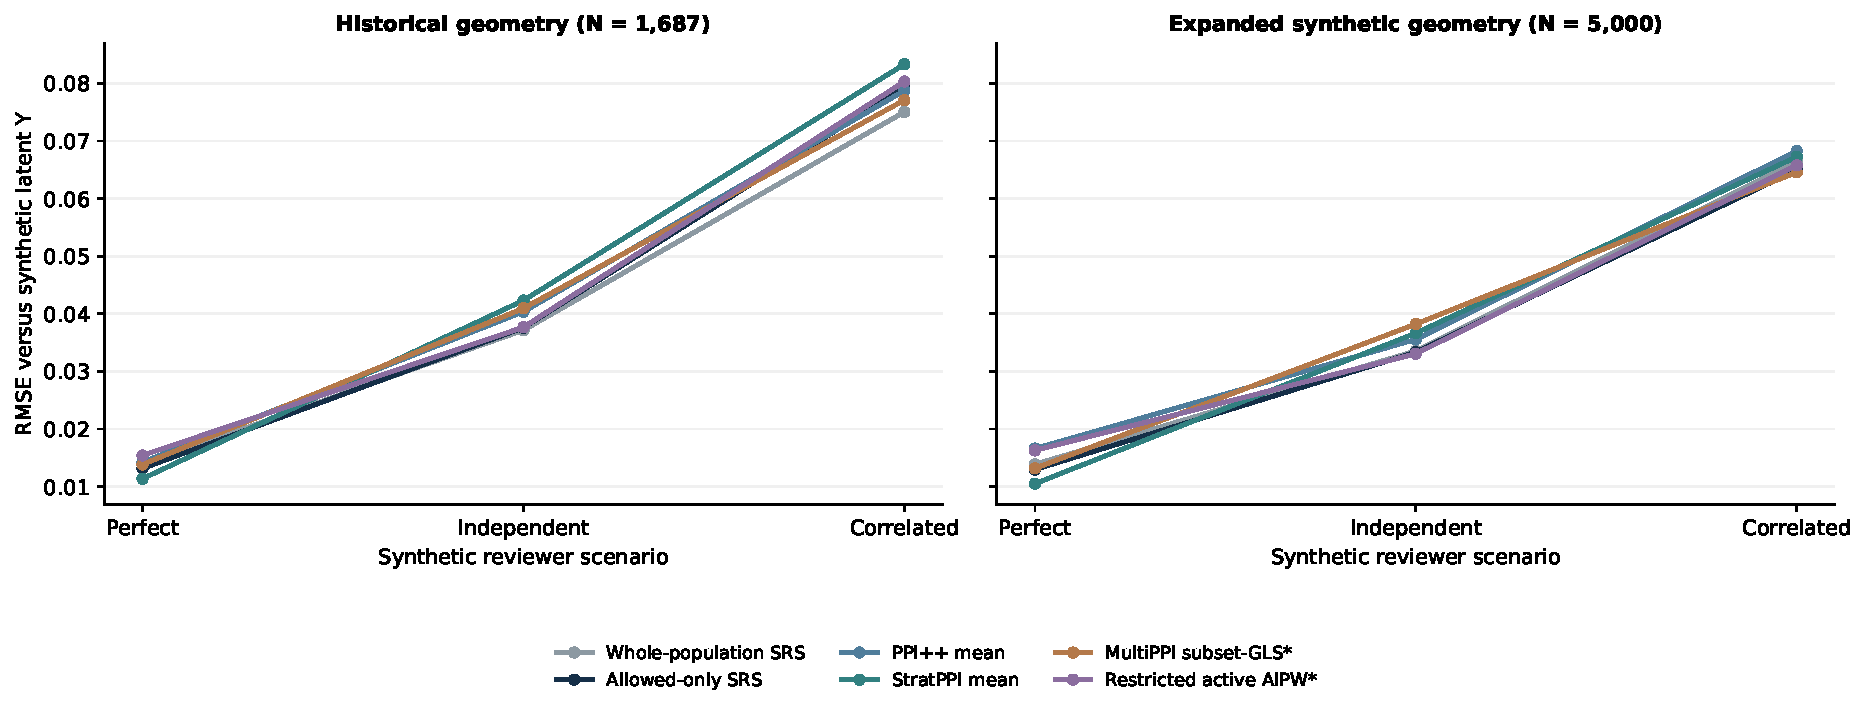
\includegraphics[width=\textwidth]{fig_cost_robustness.pdf}
\caption{Synthetic RMSE across reviewer scenarios for the latency-sensitive Phase 12B pricing model. Differences among sophisticated estimators are modest compared with changes caused by reviewer error. The baseline is not a ground-truth estimator in the real human study.}
\end{figure}

StratPPI's specialization offers a paired improvement with perfect synthetic labels: $\Delta\mathrm{RMSE}=-0.00178$ (95\% between-population bootstrap interval $[-0.00301,-0.00057]$) at $N=1{,}687$, and $-0.00246$ ($[-0.00379,-0.00087]$) at $N=5{,}000$. At $N=1{,}687$ under independent reviewer errors the difference reverses, $\Delta=+0.00472$ ($[+0.00073,+0.00857]$) [A4]. These paired intervals summarize variation across \emph{eight synthetic populations}; they do not confer external validity to real harmfulness labels. The restricted MultiPPI and active methods show no stable superiority over allowed-only SRS across these scenarios.

\subsection{Scope of the published-method comparisons}
PPI++ is a scalar-mean specialization with a charged independent pilot; StratPPI uses known strata and pilot-tuned stratum weights/allocation. Restricted MultiPPI optimizes a covariance-information proxy over nonempty subsets of \{human, cheap, expensive\} but does not match the full author's sample reuse or uncertainty theorem. The active AIPW adaptation uses with-replacement importance sampling; published AM-PPI instead jointly optimizes instance-specific predictor subset, Bernoulli label inclusion, and correction weights. The separate Bernoulli correction-identity test does not implement the full AM-PPI joint optimization. Therefore no experimental failure of the full published methods is established [A3,A5,R1--R3].

\section{Confidence intervals and allocation optimization}
\subsection{Bounded confidence intervals and coverage}
For either operational reviewer endpoint $A_Z$ or latent $A$, a known frame and monitor fraction imply $0\leq A\leq q$. If $[L,U]$ is a valid confidence interval for a \emph{fixed identified endpoint}, then $[\max(0,L),\min(q,U)]$ preserves coverage and does not increase width. We applied this transformation to intervals for the simulated reviewer-defined endpoint [A5].
\begin{table}[H]\centering\small
\caption{$N=1{,}687$, perfect simulated labels: original and support-clipped interval widths, and clipped reviewer-endpoint empirical coverage.}
\begin{tabular}{@{}lrrr@{}}\toprule
Method & Original width & Clipped width & Coverage ($Z$)\\\midrule
Allowed-only SRS & 0.0639 & 0.0639 & 0.980 \\
PPI++ mean & 0.3379 & 0.1893 & 1.000 \\
StratPPI mean & 0.4859 & 0.2628 & 1.000 \\
MultiPPI subset-GLS* & 0.3346 & 0.1877 & 1.000 \\
Restricted active AIPW* & 0.6720 & 0.3576 & 1.000 \\
\bottomrule\end{tabular}
\end{table}
\begin{figure}[H]\centering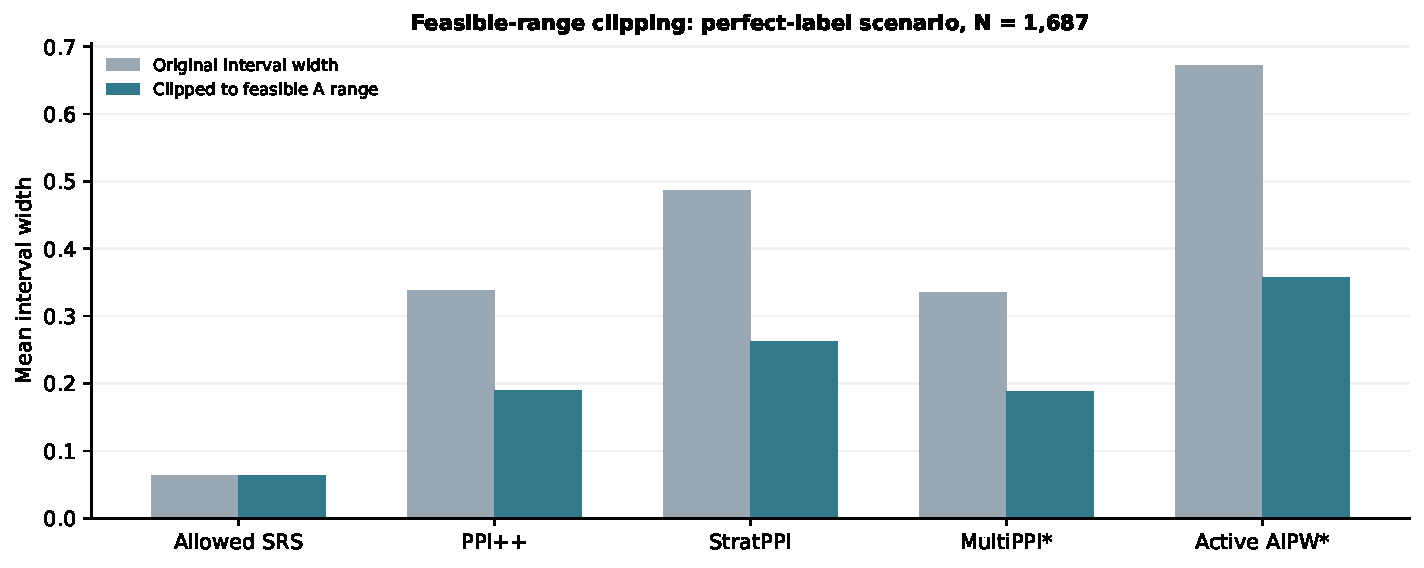
\includegraphics[width=.94\textwidth]{fig_interval_width.pdf}
\caption{Clipping narrows wide conservative intervals but does not turn them into latent-$Y$ intervals. More informative-looking exploratory Wald intervals frequently undercover.}
\end{figure}
For independent errors, the exploratory 95\% Wald interval for StratPPI has observed $Z$ coverage $0.82$ at $N=1{,}687$ and $0.835$ at $N=5{,}000$, while the clipped conservative interval's simulation coverage remains 1.0. The latter is often wide and potentially uninformative. Reviewer-$Z$ coverage is not guaranteed reviewer-$Y$ coverage under unknown misclassification.

\subsection{Numerical verification of the restricted allocation optimizer}
The restricted allocation optimizer was reimplemented with an analytic gradient and checked using a relative primal--dual gap bound, rather than relying solely on a numerical convergence flag. The criterion was \emph{certificate upper bound $\le0.5\%$}, not simply numerical solver termination. Across $2\times3\times200=1{,}200$ paired synthetic solver problems, \textbf{1,200 repaired candidates passed} and no hard-budget violations occurred [A6].
\begin{table}[H]\centering\small
\caption{Restricted allocation-optimizer comparison: restricted MultiPPI before/after repair; optimizer gap bounds are upper bounds, not realized errors.}
\begin{tabular}{@{}llrrr@{}}\toprule
$N$ & Reviewer scenario & Original RMSE & Repaired RMSE & Max repaired gap\\\midrule
1,687 & Perfect labels & 0.01385 & 0.01385 & 0.0002\% \\
1,687 & Independent noise & 0.04095 & 0.04095 & 0.0043\% \\
1,687 & Correlated noise & 0.07709 & 0.07709 & 0.0056\% \\
5,000 & Perfect labels & 0.01317 & 0.01317 & 0.0081\% \\
5,000 & Independent noise & 0.03822 & 0.03823 & 0.0031\% \\
5,000 & Correlated noise & 0.06458 & 0.06459 & 0.0024\% \\
\bottomrule\end{tabular}
\end{table}
The effect on estimation RMSE is negligible despite the improved numerical certificate.

\section{Observed review time and model latency}
The existing historical 128-case component benchmark directly measured mean/p95 latencies; a separate 363-case T4 policy benchmark was not pooled with it [A4,D1].
\begin{table}[H]\centering\small
\caption{Historical runtime component measurements; not contemporaneous selected-case economic costs.}
\begin{tabular}{@{}lrrr@{}}\toprule
Component & Mean (ms) & p95 (ms) & $n$\\\midrule
Rule-based filter & 1.271 & 2.595 & 128\\
Koala compact moderation & 45.657 & 70.655 & 128\\
Qwen3Guard generation-based & 1,597.561 & 2,431.597 & 128\\\bottomrule
\end{tabular}
\end{table}
Economic equality cannot be inferred from equal numerical wall seconds: GPU execution, human attention, preparation, latency tails and review adjudication have different costs and can run asynchronously. The ledger used for synthetic method comparison is
\begin{equation}
 C_{\mathrm{total}}=C_{\mathrm{human,cal}}+C_{\mathrm{human,eval}}+n_c c_c+n_e c_e+C_{\mathrm{organize}}+C_{\mathrm{adjudicate}}+C_{\mathrm{other}}.
\end{equation}
Only the first four terms were actively charged in the controlled simulations, with proxy rates mapped by an assumed conversion; $C_{\mathrm{organize}}$, $C_{\mathrm{adjudicate}}$ and $C_{\mathrm{other}}$ remain unmeasured rather than set to zero in claims about real economic parity. Actual new selected-case native-monitor execution and verified wages/hardware charges are not available. The unit-ratio sensitivity comparison examines a cost model; it is not an accounting of monetary expenditure.

\section{Relation to prior work and limitations}
\begin{table}[H]\centering\scriptsize
\caption{Research overlap and the unestablished gap; these references motivated the fidelity check.}
\begin{tabularx}{\textwidth}{@{}p{0.25\textwidth}X@{}}\toprule
Literature & Why the present project cannot claim the component as new\\\midrule
StratPPI (Fisch et al., 2024) & Stratified prediction-powered estimation and confidence regions already studied [R1].\\
MultiPPI (Cowen-Breen et al., 2026) & Heterogeneous multi-predictor measurement allocation and theoretical uncertainty already studied [R2].\\
AM-PPI (Brawand et al., 2026) & Instance-level acquisition, Bernoulli human sampling, and weighted correction already studied [R3].\\
Online Safety Monitoring (Schirmer et al., 2026) & Risk-controlled online alarm thresholds; a different estimand but relevant safety-monitor inference [R4].\\
Noisy but Valid (Feng et al., 2026) & Imperfect-judge reliability/calibration; cannot claim generic noise correction as novel [R5].\\
Safer or Luckier? (Chen and Goldfarb-Tarrant, 2025) & Sensitive safety evaluation and judge disagreement are known issues [R6].\\\bottomrule
\end{tabularx}
\end{table}
The results highlight the combined effect of costly reviews, heterogeneous response-level judgments, and proxy-assisted sampling. The results cannot currently show (i) true latent-$Y$ prevalence from the 96 cases, (ii) author-equivalent MultiPPI/AM-PPI performance, (iii) a genuine money-matched efficiency advantage, (iv) distribution-shift resilience, or (v) a validated native-monitor deployment. The earlier final-test and shift data were already historically accessed and are \emph{not} fresh confirmatory data. The old v2 result has incomplete final-table timing provenance, and historical singleton-style grouping cannot prove independence [D1].

\section{Discussion and further work}
\textbf{Research direction.} \emph{When can response-level missed-harm prevalence be identified and estimated at useful precision under heterogeneous, possibly correlated human safety judgments and bounded review cost?} Further methodological work would need to identify a precise statistical problem that is not already resolved by existing methods for noisy labels, stratified sampling, or prediction-powered inference. The current observations also support a narrower empirical account of measurement reliability and sampling cost.

\textbf{Proposed prospective evaluation.} With approval and permissions, freeze one target assistant, a native post-generation monitor, exact C1--C8 policy and a fresh response frame. Draw separate simple random samples \emph{without replacement} from \textbf{allowed and blocked} strata with precommitted inclusion probabilities; obtain two independent policy-blinded human assessments, preserve Uncertain, predefine a third adjudicator for disagreements and measure active/wall, organizer, inference and adjudication costs. Estimate an operational reviewer-defined $A_{Z^*}$ by
\begin{equation}\label{eq:finite}
 \widehat A_{Z^*}=\frac{N_0}{N}\cdot\frac{1}{n_0}\sum_{i\in S_0} Z_i^*, \qquad \pi_i=n_0/N_0\quad (D_i=0),
\end{equation}
with design-based finite-population uncertainty only for an identified fixed reference endpoint $Z^*$. Blocked cases support decomposition and FNR/FPR diagnostics. Any unresolved judgments require transparent intervals or bounds; this is \emph{not} an interval for latent $Y$ without additional validated assumptions. The current sampling prototype covers only allowed responses and requires extension to the blocked stratum before use in a prospective study. No new reviewer judgments or fresh native-response frame have been collected [A7].

\textbf{Open questions.} Two issues remain unresolved: whether one can identify and estimate $A$ with useful precision under correlated and potentially biased human judgments, and what review-and-inference budget is needed to do so. A small prospective study would help quantify the disagreement and cost components on a fresh native-monitor sample. The appropriate next step is to decide whether to prioritize an identification result, an empirical measurement study, or both, before extending data collection.

\section{Reproducibility and data access}
The accompanying source package includes executable code for the estimator comparisons, interval calculations, optimizer verification, and proposed reference-sampling procedure, together with selected aggregate results, test suites, and the LaTeX report source. In the audited package, $10+10+12+9=41$ tests passed using synthetic fixtures; aggregate consistency checks also passed. This number describes automated software checks, \emph{not} proof of statistical validity or reviewer correctness. The code distinguishes restricted estimator implementations from the corresponding full published methods.

Private SQL databases, raw case texts, case mappings, individual human votes, reviewer notes, reviewer credentials and complete private policy snapshots remain local. The repository's older routing results and negative experiment evidence are unchanged. Local evidence hashes and population provenance are recorded, but the uploaded aggregate summaries cannot independently reconstruct private observations.

\section{Conclusion}
In the historical development comparison, the reduction in observed harmful allowed responses from selective Qwen acquisition was small. Simple random sampling performed competitively with the restricted prediction-powered estimators, and the human-review study showed that disagreement between raters was too large to treat a single reviewer\'s verdict as ground truth. Interval and optimization checks improved numerical reliability but did not resolve the missing reference-outcome problem. A small fresh, independently reviewed sample with documented costs would clarify the practical limits of missed-harm estimation, provided a specific scientific objective is agreed before collection.

\section*{References and data sources}
\footnotesize
\begin{description}[leftmargin=7mm,labelwidth=6mm,labelsep=0mm,itemsep=0pt,topsep=2pt]
\item[{[D1]}] Trustworthy AI project repository: \href{https://github.com/tivdzualubem/trustworthy-ai-monitor-fusion}{GitHub repository}; historical evaluation and latency summaries on the development branch, accessed Nov. 2026.
\item[{[A1]}] Retrospective monitor-decision and baseline-sampling analysis, aggregate results and code, 2026.
\item[{[A2]}] Human-review study: 96-case agreement and active-duration summaries; private individual judgments retained locally, 2026.
\item[{[A3]}] Cost-controlled estimator comparison: synthetic benchmark, two population geometries, aggregate outputs and implementation, 2026.
\item[{[A4]}] Measured component-latency summaries and cost-sensitivity analysis; component benchmark $n=128$ and separate T4 policy benchmark $n=363$, 2026.
\item[{[A5]}] Confidence-interval and estimator identity checks: methods, simulations and numerical results, 2026.
\item[{[A6]}] Restricted MultiPPI allocation-optimizer verification and paired evaluation, 2026.
\item[{[A7]}] Prospective response-review sampling and adjudication protocol with software tests; no new cases reviewed, 2026.
\item[{[R1]}] Fisch et al., \emph{Stratified Prediction-Powered Inference}, NeurIPS 2024. \url{https://arxiv.org/abs/2406.04291}
\item[{[R2]}] Cowen-Breen et al., \emph{Multiple-Prediction-Powered Inference}, ICLR 2026. \url{https://arxiv.org/abs/2603.27414}
\item[{[R3]}] Brawand et al., \emph{Active Multiple-Prediction-Powered Inference}, 2026 preprint. \url{https://arxiv.org/abs/2605.08429}
\item[{[R4]}] Schirmer et al., \emph{Online Safety Monitoring for LLMs}, 2026 preprint. \url{https://arxiv.org/abs/2607.02510}
\item[{[R5]}] Feng et al., \emph{Noisy but Valid: Robust Statistical Evaluation of LLMs with Imperfect Judges}, ICLR 2026. \url{https://arxiv.org/abs/2601.20913}
\item[{[R6]}] Chen and Goldfarb-Tarrant, \emph{Safer or Luckier?}, ACL 2025. \url{https://aclanthology.org/2025.acl-long.970/}
\end{description}
\end{document}
